\documentclass[a4paper,12pt]{report} % добавить leqno в [] для нумерации слева

%%% Работа с русским языком
\usepackage{cmap}					% поиск в PDF
\usepackage{mathtext} 				% русские буквы в формулах
\usepackage[T2A]{fontenc}			% кодировка
\usepackage[utf8]{inputenc}			% кодировка исходного текста
\usepackage[english,russian]{babel}	% локализация и переносы

%%% Дополнительная работа с математикой
\usepackage{amsmath,amsfonts,amssymb,amsthm,mathtools} % AMS
\usepackage{icomma} % "Умная" запятая: $0,2$ --- число, $0, 2$ --- перечисление

%% Номера формул
\mathtoolsset{showonlyrefs=true} % Показывать номера только у тех формул, на которые есть \eqref{} в тексте.

%% Шрифты
\usepackage{euscript}	 % Шрифт Евклид
\usepackage{mathrsfs} % Красивый матшрифт

%% Свои команды
\DeclareMathOperator{\sgn}{\mathop{sgn}}

%\setlength\parindent{0ex}
%\setlength\parskip{0.3cm}

%%% Заголовок
\author{Волков Павел А-14-19}
\title{Типовой расчет №13 по численным методам Вариант 3}
\date{\today}

\usepackage{graphicx}

\begin{document} % конец преамбулы, начало документа

\maketitle

\newpage
\section*{Задание}

Функция $y = y(x)$ задана таблицей своих значений. Применяя метод наименьших квадратов, проблизить функцию многочленами 1-й и 2-й степеней. Для каждого приближения определить величину среднеквадратичной погрешности. Построить на одном чертеже точечный график функции и графики многочленов
\[
\begin{tabular}{ | c | c | c | c | c | c |}
	\hline
	$x$ & -1.4 & -0.7 & 0 & 0.7 & 1.4 \\ \hline
	$y$ & 2.5 & 5.4 & 7.3 & 3.9 & 1.8 \\ \hline
\end{tabular}
\]

\section*{Решение}

Приблизим функцию многочленом 1-й степени: $P_1(x) = a_0 + a_1x$. Нормальная система наименьших квадратов при этом имеет вид:
\[
	\left\{
		\begin{aligned}
		s_0a_0 + s_1a_1 = b_0  \\
		s_1a_0 + s_2a_1 = b_1 \\
		\end{aligned}
	\right.
\]
Вычислим все коэффициенты
\begin{gather}
	s_0 = \sum\limits_{i = 0}^n x_i^0 = 5 \\
	s_1 = \sum\limits_{i=0}^n x_i^1 = 0 \\
	s_2 = \sum\limits_{i = 0}^n x_i^2 = 4.9 \\
	b_0 = \sum\limits_{i=0}^n y_ix_i^0 = 20.9 \\
	b_1 = \sum\limits_{i=0}^n y_ix_i^1 = -2.03 \\
\end{gather}

Таким образом, система принимает вид:

\[
	\left\{
		\begin{aligned}
		5a_0 = 20.9  \\
		4.9a_1 = -2.03 \\
		\end{aligned}
	\right.
\]
$P_1(x) = 4.18 + 0.414x$

Вычислим значения многочлена в узлах таблицы: $P_1(-1.4) = 3.6$, $P_1(-0.7) = 3.89$, $P_1(0) = 4.18$, $P_1(0.7) = 4.47$, $P_1(1.4) = 4.76$

Тогда $\sigma(P_1, f) = 2.112$

Теперь приблизим функцию многочленом 2-й степени: $P_2(x) = a_0 + a_1x + a_2x^2$.

\[
	\left\{
		\begin{aligned}
		s_0a_0 + s_1a_1 + s_2a_2= b_0  \\
		s_1a_0 + s_2a_1 + s_3a_2= b_1 \\
		s_2a_0 + s_3a_1 + s_4a_2 = b_2
		\end{aligned}
	\right.
\]
Вычислим недостающие коэффициенты системы: $s_3 = 0$, $s_4 = 8.1634$, $b_2 = 12.985$

И получим следующий многочлен: $P_2(x) = 6.366 - 0.414x-2.230x^2$ со среднеквадратичным отклонением $\sigma(P_2, f) = 0.667$.

Графики представленных функций:

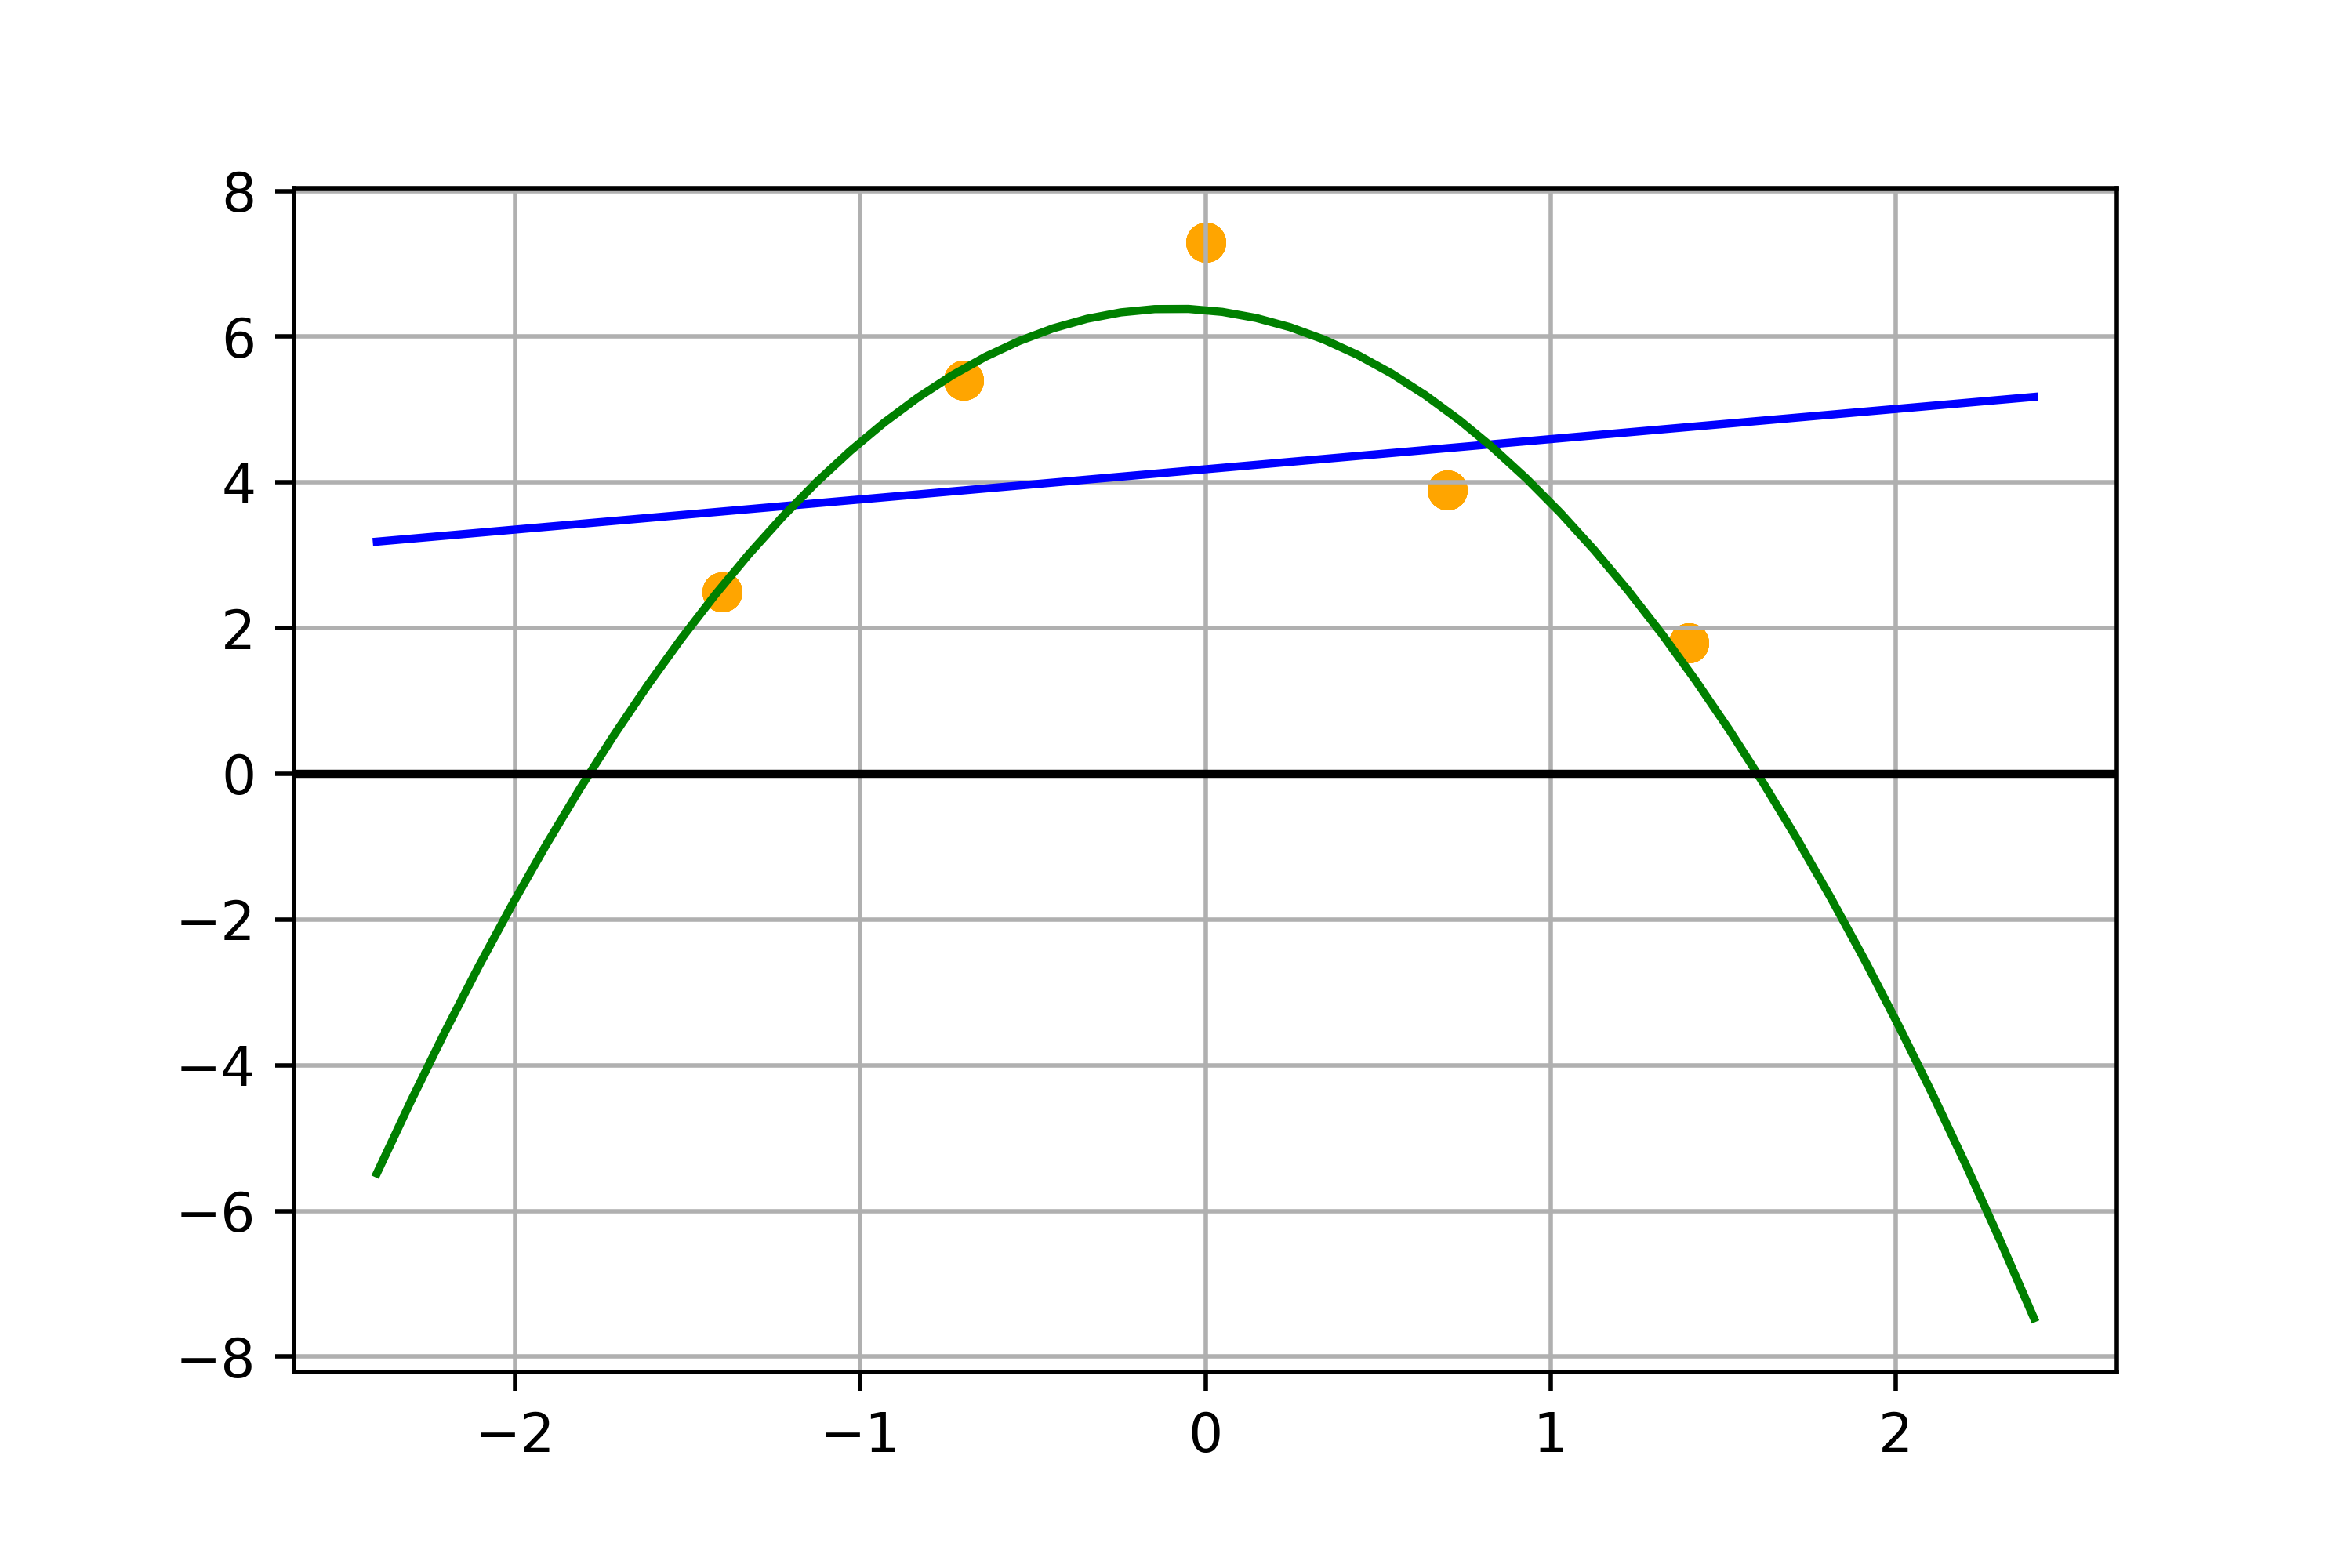
\includegraphics{regular_calc_13.png}

\end{document}